\documentclass{article}

\usepackage[margin=4cm]{geometry}
\usepackage{polyglossia}
	\setmainlanguage{english}
\usepackage{amsmath}
\usepackage{amssymb}
\usepackage{siunitx}
\usepackage{float}
\usepackage{booktabs}
\usepackage{subcaption}
\usepackage{graphicx}
\usepackage{xcolor}
\usepackage{listings}
    \lstset{language=Python,
	basicstyle=\footnotesize\ttfamily,
	breaklines=true,
	framextopmargin=50pt,
	frame=bottomline,
	backgroundcolor=\color{white!85!black},
	commentstyle=\color{blue},
	keywordstyle=\color{red},
	stringstyle=\color{orange!80!black}}
\usepackage{tikz}

\title{Computational Physics - Exercise 7}
\author{Maurice Donner \and Lukas Häffner}

\begin{document}

\maketitle
\newpage

\section{Many Species Population Dynamics}

Given are 3 predator (\( P \)) and 3 prey (\( N \)) species, that change
according to the following equations:

\begin{align}
    \frac{d\mathbf{N}}{dt} = \mathbf{N} \cdot \left( \mathbf{a} -
    \mathbf{\hat b \cdot P} \right), \quad
    \frac{d\mathbf{P}}{dt} = \mathbf{P} \cdot \bigg( 
    \mathbf{\hat c \cdot N} - \mathbf{d} \bigg)
\end{align}

With \( \mathbf{a, d, \hat b, \hat c} \) being the following vectors/matrices:

% {{{ Vectors and Matrices
\begin{align}
    \mathbf{a} =
    \left(
	\begin{matrix}
	    55 \\ 
	    34 \\
	    11	 
	\end{matrix}
    \right) &, \quad
    \mathbf{d} =
    \left(
	\begin{matrix}
	    85 \\ 
	    9 \\
	    35 
	\end{matrix}
    \right) \\[.5cm]
    \mathbf{\hat b} = 
    \left(
	\begin{matrix}
	    20 & 30 & 5 \\ 
	    1 & 3 & 7 \\
	    4 & 10 & 20 
	\end{matrix}
    \right) &, \quad
    \mathbf{\hat c} =
    \left(
	\begin{matrix}
	    20 & 30 & 35 \\ 
	    3 & 3 & 3 \\
	    7 & 8 & 20 
	\end{matrix}
    \right)
\end{align}
% }}}

Solving \( \frac{d \mathbf{N/P}}{dt} = 0 \) yields the following stationary
points:

\begin{align}
    \mathbf{N_1^{*}} = \left( \begin{matrix} 0 \\ 0 \\ 0 \end{matrix} \right),
    \mathbf{N_2^{*}} = \left( \begin{matrix} 1 \\ 1 \\ 1 \end{matrix} \right),
    \mathbf{P_1^{*}} = \left( \begin{matrix} 0 \\ 0 \\ 0 \end{matrix} \right),
    \mathbf{P_2^{*}} = \left( \begin{matrix} 1 \\ 1 \\ 1 \end{matrix} \right),
    \label{stationary}
\end{align}

Calculating the Jacobi-Matrix at the non-trivial stationary point:

\begin{align}
    \mathbf{\hat A} =
    \left(
	\begin{matrix}
	    \left. \dfrac{\partial}{\partial \mathbf{N}} \left(
	    \dfrac{d \mathbf{N}}{dt} \right) \right| 
	    _{\mathbf{N^*_2}, \mathbf{P^*_2}}
	    & \left. \dfrac{\partial}{\partial \mathbf{P}} \left( 
	    \dfrac{d \mathbf{N}}{dt} \right) \right| 
	    _{\mathbf{N^*_2}, \mathbf{P^*_2}} \\[2ex]
	    \left. \dfrac{\partial}{\partial \mathbf{N}} \left(
	    \dfrac{d \mathbf{P}}{dt} \right) \right|
	    _{\mathbf{N^*_2}, \mathbf{P^*_2}}
	    & \left. \dfrac{\partial}{\partial \mathbf{P}} \left(
	    \dfrac{d \mathbf{P}}{dt} \right) \right|
	    _{\mathbf{N^*_2}, \mathbf{P^*_2}}
	\end{matrix}
    \right) = 
    \left(
	\begin{matrix}
	    \mathbf{a - \hat b \cdot P} & \mathbf{-N \cdot \hat b} \\ 
	    \mathbf{P \cdot \hat c} & \mathbf{\hat c \cdot n - d} 
	\end{matrix}
    \right)
\end{align}

But with (\ref{stationary}) we know that \( \mathbf{a - \hat b \cdot P} =
    0
= \mathbf{\hat c \cdot N - d} .
\) 
So \( \mathbf{\hat A} \) reduces to:

\begin{align}
    \mathbf{\hat A} = 
    \left(
	\begin{matrix}
	    0 & - \mathbf{\hat b} \\
	    \mathbf{\hat c} & 0
	\end{matrix}
    \right) = %second matrix
    \left( \begin{matrix}
    0 &
    - \left(
	\begin{matrix}
	    20 & 30 & 5 \\ 
	    1 & 3 & 7 \\
	    4 & 10 & 20 
	\end{matrix}
    \right) \\
    \left(
	\begin{matrix}
	    20 & 30 & 35 \\ 
	    3 & 3 & 3 \\
	    7 & 8 & 20 
	\end{matrix}
    \right) & 0
    \end{matrix} \right)
\end{align}

Solving this with numpy function \texttt{numpy.linalg.eig} gives us the wanted
eigenvalues and eigenvectors:

\begin{table}[H]
    \centering
    \begin{tabular}{rll}
	\toprule 
& Eigenvalue & Eigenvector \\ \midrule
&33.63i & (0.54i, 0.54i, 0.87, 0.87, -0.23, 0.23 \\ 
-&33.63i & (0.09i, -0.09i, -0.14, -0.14, 0.13i, -0.13i) \\ 
&7.7i & (0.29i -0.29i, -0.034, -0.34, 0.03, -0.03)  \\ 
-&7.7i & (0.71, 0.71, -0.17i, 0.17i,-0.79 -0.79) \\ 
-&0.39 & (0.08, 0.0, -0.15i, 0.15i, 0.54, 0.54) \\ 
&0.39 & (0.31, 0.31, 0.24i, -0.24i, -0.11, -0.11)\\
\bottomrule 
\end{tabular}
\caption{Eigenvalues and Eigenvectors of Jacobi Matrix A}
\end{table}

Choosing an initial state \( \mathbf{n} = \sum_{^{6} _{\text{i=1}}}
    c_i \mathbf{v}_i \) with \( c = (3,3,1,1,5,0.1) \)
\[ 
    \mathbf{n} = (1.16+2.2i, 1.16-2.2i, 1.85-0.9i, 1.85+0.9i, 1.63, 2.19)
\]

We plot the temporal evolution of all 6 populations:
\begin{figure}[ht]
    \centering
    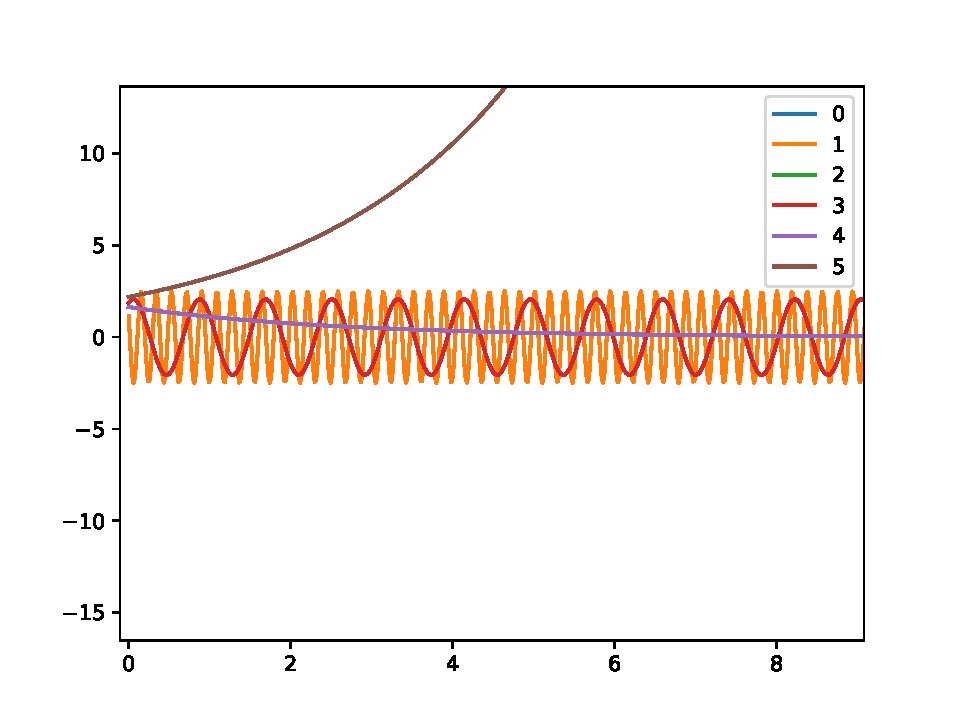
\includegraphics[width=9cm]{Populations.pdf} 
    \caption{Temporal evolution of the 3 prey (0,1,2) and 3 predator 
	(3,4,5) populations} 
\end{figure}
\end{document}

